% ========== 2023年07月06号 第**次课 应用 ==========

%\frame{\titlepage}

\section{应用*}


\title{第十一章 \quad 应用*}
\author{}
\date{}

\makeatletter
\ifodd\value{page}
    \frame{\titlepage}
\else
    \frame{\mbox{}}
    \frame{\titlepage}
\fi
\makeatother



\subsection{桁架的静力分析*}
\begin{frame}\frametitle{桁架的静力分析*}

    桁架是一种由直杆铰接而成的空间结构, 杆件主要承受轴向拉力和压力. 例如:屋顶、桥梁、塔架等.

    \begin{figure}
    \centering
    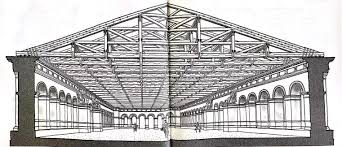
\includegraphics[width=0.3\linewidth]{pic/屋顶}
    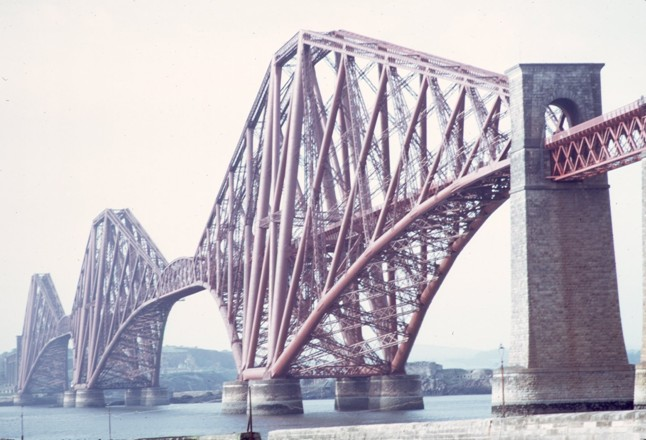
\includegraphics[width=0.3\linewidth]{pic/桥}
    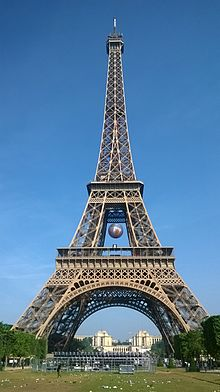
\includegraphics[width=0.3\linewidth]{pic/塔}
    \end{figure}
    \end{frame}






\begin{frame}\frametitle{桁架的静力分析*}
    \begin{question}
    考虑如下桁架的简化模型. 各个直杆长度相同,忽略桁架自重.
    在 $B$处施以一个大小为$F$的向下的力.求各个直杆所承受的力.
    \end{question}

% 定义自定义样式
\tikzset{
  line/.style={draw, thick}, % 定义线条样式
  dot/.style={circle, fill, inner sep=1.5pt}, % 定义点样式
  dot label/.style={font=\scriptsize} % 定义标签样式
}
    \begin{center}
    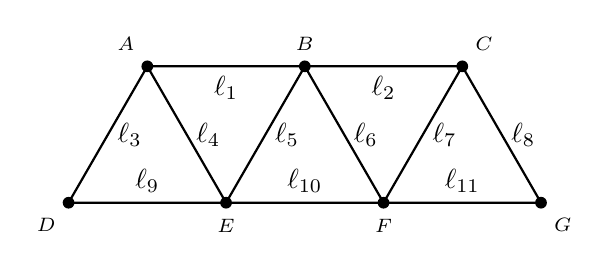
\begin{tikzpicture}
    \coordinate (A) at (-2,1.732);
    \coordinate (B) at (0,1.732);
    \coordinate (C) at (2,1.732);
    \coordinate (D) at (-3,0);
    \coordinate (E) at (-1,0);
    \coordinate (F) at (1,0);
    \coordinate (G) at (3,0);

    \node at (-1,1.732) [below] {$\ell_1$};
    \node at (1,1.732) [below] {$\ell_2$};
    \node at (-2.5,0.866) [right] {$\ell_3$};
    \node at (-1.5,0.866) [right] {$\ell_4$};
    \node at (-0.5,0.866) [right] {$\ell_5$};
    \node at (0.5,0.866) [right] {$\ell_6$};
    \node at (1.5,0.866) [right] {$\ell_7$};
    \node at (2.5,0.866) [right] {$\ell_8$};
    \node at (-2,0) [above] {$\ell_9$};
    \node at (0,0) [above] {$\ell_{10}$};
    \node at (2,0) [above] {$\ell_{11}$};

    \draw[line]
    (A)--(B)--(C)--(G)--(F)--(E)--(D)--(A)--(E)--(B)--(F)--(C);
    \foreach \i/\angle in {A/120,B/90,C/60,D/-120,E/-90,F/-90,G/-60} {
    \node[dot, label={[dot label]\angle:$\i$}] at (\i) {};
      }
    \end{tikzpicture}
    \end{center}
    \end{frame}






\begin{frame}\frametitle{桁架的静力分析*}
    解:记杆$\ell_i$受到大小为$f_i$的压力(压力为负,则表示受到拉力). 根据各节点处杆件的平衡条件可得
    \begin{equation*}
    \left\{\begin{array}{lll}
    (P_1):& -f_1+\frac12(f_3-f_4)=0,& f_3+f_4=0;\\
    (P_2):& f_1-f_2=0,&\frac{\sqrt{3}}{2}(f_5+f_6)=F;\\
    (P_3):& f_2+\frac12(f_7-f_8)=0,&f_7+f_8=0;\\
    (P_5):&f_4+f_5=0 &\frac12(f_4-f_5)+f_9-f_{10}=0;\\
    (P_6):&f_6+f_7=0 &\frac12(f_6-f_7)+f_{10}-f_{11}=0;\\
    (P_4,P7):&\frac12f_3+f_9=0, &\frac12f_8+f_{11}=0\\
    \end{array}\right.
    \end{equation*}
    \end{frame}





\subsection{电网络分析*}
\begin{frame}\frametitle{电网络分析*}
    \begin{question}
    考虑如下RLC电路图.已知 $R_1=1\Omega$, $R_2=3\Omega$, $\epsilon=3V$, $C=0.5F$, $L=5H$.设初始开关断开,各支路电流都为零.
    \begin{figure}
    \centering
    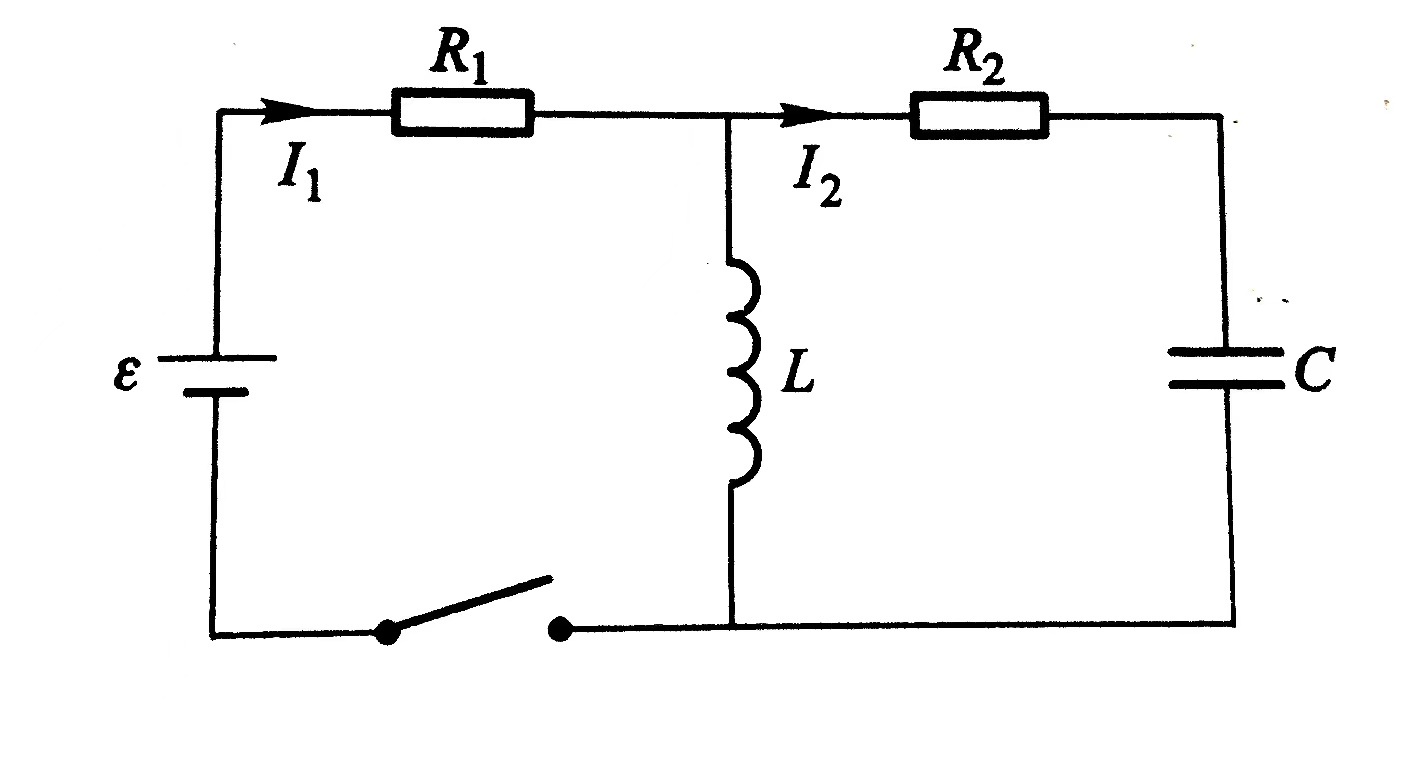
\includegraphics[width=0.4\linewidth]{pic/电路图}
    \end{figure}
    求开关闭合后两个支路的电流$I_1(t)$和$I_2(t)$随时间的变化.
    \end{question}
    解: 根据Krichhoff定律和Phm定律,可得微分方程组:
    \begin{equation*}
    \left\{
    \begin{array}{l}
    L(I_1(t)-I_2(t))' = \epsilon - R_1I_1(t)\\
    C(\epsilon-R_1I_1(t)-R_2I_2(t))' = I_2(t) \\
    I_1(0) = I_2(0) = 0\\
    \end{array}
    \right.
    \end{equation*}\end{frame}






\begin{frame}\frametitle{电网络分析*}
    于是
    \begin{equation*}
    \begin{pmatrix}I_1'(t)\\I_2'(t)\\\end{pmatrix}
    =\begin{pmatrix}-\frac{3}{20}&-\frac12\\\frac1{20}&-\frac12\\\end{pmatrix}
    \begin{pmatrix}I_1(t)-3\\I_2(t)\\\end{pmatrix}
    \end{equation*}
    解得
    \[\begin{pmatrix}I_1(t)-3\\I_2(t)\\\end{pmatrix} = e^{At}\begin{pmatrix}-3\\0\\\end{pmatrix}\]
    其中
    \[A=\begin{pmatrix}-\frac{3}{20}&-\frac12\\\frac1{20}&-\frac12\\\end{pmatrix}
    =\begin{pmatrix}2&5\\1&1\\\end{pmatrix} \begin{pmatrix}-\frac25&\\&-\frac14\\\end{pmatrix}\begin{pmatrix}2&5\\1&1\\\end{pmatrix}^{-1}\]
    \[e^{At}=\sum_{n=0}^{\infty}\frac{t^n}{n!}A^n=\begin{pmatrix}2&5\\1&1\\\end{pmatrix} \begin{pmatrix}e^{-\frac{2t}5}&\\&e^{-\frac{t}4}\\\end{pmatrix}\begin{pmatrix}2&5\\1&1\\\end{pmatrix}^{-1}\]
    从而,得
    \begin{equation*}
    \left\{
    \begin{array}{l}
    I_1(t) = 3 +2e^{-\frac{2t}{5}} - 5e^{-\frac{t}{4}}\\
    I_2(t) = e^{-\frac{2t}{5}} - e^{-\frac{t}{4}}\\
    \end{array}
    \right.
    \end{equation*}
    \end{frame}





    \subsection{多项式公因子与方程求解*}
\begin{frame}\frametitle{多项式公因子与方程求解*}
    给定两个一元多项式
    \[f(x)=a_0+a_1x+\cdots+a_mx^m,\quad g(x)=b_0+b_1x+\cdots+b_nx^n,\quad (a_mb_n\neq0).\]
    \begin{question}
    在不做因式分解和不求这两个多项式的根的情况下,如何判断它们是否有公因子或公共根?
    \end{question}
    称方阵 $S=\begin{pmatrix}
    a_0 &&& b_0&&\\
    a_1 &\ddots&& b_1&\ddots&\\
    \vdots &\ddots&a_0& \vdots&\ddots&b_0\\
    a_m &&a_1& b_m&&b_1\\
     &\ddots&\vdots&&\ddots& \vdots\\
    &&a_m&&&b_m\\
    \end{pmatrix} $
    为$f(x)$和$g(x)$的Sylvester矩阵.称其行列式$Syl(f,g):=\det(S)$为Sylvester结式.
    \begin{theorem}
    多项式$f(x)$和$g(x)$有公因子,当且仅当$\det(S)=0$.
    \end{theorem}
    \end{frame}






\begin{frame}\frametitle{多项式公因子与方程求解*}
    证明思路:这是由于$f(x)$和$g(x)$有公因子,当且仅当存在非零多项式$A(x)=A_0+A_1x+\cdots+A_{n-1}x^{n-1}$和$B(x)=B_0+B_1x+\cdots+B_{m-1}x^{m-1}$使得
    \[A(x)f(x)+B(x)g(x)=0\qquad(**)\]
    计算$(**)$中的系数得
    \[\begin{pmatrix}
    a_0 &&& b_0&&\\
    a_1 &\ddots&& b_1&\ddots&\\
    \vdots &\ddots&a_0& \vdots&\ddots&b_0\\
    a_m &&a_1& b_m&&b_1\\
     &\ddots&\vdots&&\ddots& \vdots\\
    &&a_m&&&b_m\\
    \end{pmatrix}
    \begin{pmatrix}A_0\\\vdots\\A_{n-1}\\B_0\\\cdots\\B_{m-1}\\\end{pmatrix}=0\qquad(***)\]
    而齐次方程$(***)$有解当且仅当$\det(S)=0$.
    \end{frame}





    \subsection{组合与图论*}
\begin{frame}\frametitle{组合与图论*}
    \begin{question}
    假设 $m$个学生组织了 $n$次集体活动, 每次至少 $2$人参加, 并且任意 $2$个同学一起参加的活动恰有 $1$次. 求证: $n=1$或者$m\leq n$.
    \end{question}
    解: 令 $A=(a_{ij})_{m\times n}$, 其中若学生$i$参加了活动$j$则$a_{ij}=1$,否则$a_{ij}=0$. 由题意知
    \[AA^T = \begin{pmatrix} t_1 & 1&\cdots&1\\1&t_2&\ddots&\vdots\\\vdots&\ddots&\ddots&1\\1&\cdots&1&t_m\\\end{pmatrix}_.\]
    其中$t_i$为学生$i$参加活动总次数.

    分情况讨论:
    \begin{itemize}
    \item 若 $t_i=1$,则 $n=1$;
    \item 若对所有$i$,$t_i\geq2$.则 $AA^T>0$.因此$A$行满秩,从而$m\leq n$.
    \end{itemize}
    \end{frame}






\begin{frame}\frametitle{组合与图论*}
    \begin{question}[关灯游戏]
    在$m\times n$的棋盘中每个方格内均设置一盏灯和一个按钮. 当某个方格内的按钮被按动后,这个方格内的灯将从亮变灭或从灭变亮,与这个方格有公共边的方格内的灯也将同样的变化.假设初始时每盏灯都是亮的,问是否可以按下一些列的按钮使得最终所有灯都变灭.
    \end{question}
    解题思路: 灯的状态可用$\mathbb F_2^N$中的向量代表.每个按钮也都看成$\mathbb F_2^N$中的一个向量$\alpha_i$.则问题转化为判定
    $\textbf{1}=(1,1,\cdots,1)^T$是否落在$\{\alpha_1,\cdots,\alpha_{mn}\}$生成子空间$V$中.

    令$A=(\alpha_1,\cdots,\alpha_{mn})$,则 $A$对称且对角线全为$1$. 从而
    \[y^TAy =\textbf{1}^Ty.\]
    因此与$V$正交的向量都与$\textbf{1}$正交. 从而$\textbf{1}\in V$. 也就是说可以经过一些列的按钮使得最终所有灯都变灭.

    \bigskip

    注: 组合数学和图论中的许多问题都可以转化为矩阵问题处理.
    \end{frame}





    \subsection{多元函数的极值*}
\begin{frame}\frametitle{多元函数的极值*}
    设$\textbf{x}=(x_1,\cdots,x_n)$是$n$个变量, $f(\textbf{x})$是定义在区域$D\subseteq R^n$上的$n$元光滑函数.根据Taylor公式
    \[f(\textbf{x}) = f(\textbf{a}) +J(\textbf{a})(\textbf{x}-\textbf{a}) + \frac12(\textbf{x}-\textbf{a})^T\textbf{H}(\textbf{a})(\textbf{x}-\textbf{a})+o(|\textbf{x}-\textbf{a}|^2),\]
    其中
    \[J(\textbf{x}) = \left(\frac{\partial f(\textbf{x})}{\partial x_1},\cdots,\frac{\partial f(\textbf{x})}{\partial x_n}\right)\qquad \text{Jacobi 矩阵}\]
    和
    \[H(\textbf{x}) = \begin{pmatrix}
    \frac{\partial^2 f(\textbf{x})}{\partial x^2_1} & \cdots & \frac{\partial^2 f(\textbf{x})}{\partial x_1\partial x_n}\\
    \vdots&&\vdots\\
    \frac{\partial^2 f(\textbf{x})}{\partial x_n\partial x_1} & \cdots & \frac{\partial^2 f(\textbf{x})}{\partial x_n^2}\\
    \end{pmatrix} \qquad \text{Hesse 矩阵}.\]

    \begin{theorem}假设同上. 则有
    \begin{itemize}
    \item 设 $f(x)$ 在 $\textbf{a}$ 处达到极小(大)值, 则$J(\textbf{a}) =0$且$H(\textbf{a})\geq0(\leq0)$.
    \item 若$J(\textbf{a}) =0$且$H(\textbf{a})>0(<0)$,则$f(x)$ 在 $\textbf{a}$ 处达到极小(大)值.
    \end{itemize}
    \end{theorem}
    \end{frame}





    \subsection{计算机绘图与图像变换*}
\begin{frame}\frametitle{计算机绘图与图像变换*}
    在计算机中,无论是二维平面图形还是三维立体图形,都需要通过图形变换,把图形变换到显示器屏幕上,然后显示出来.
    \begin{figure}
    \centering
    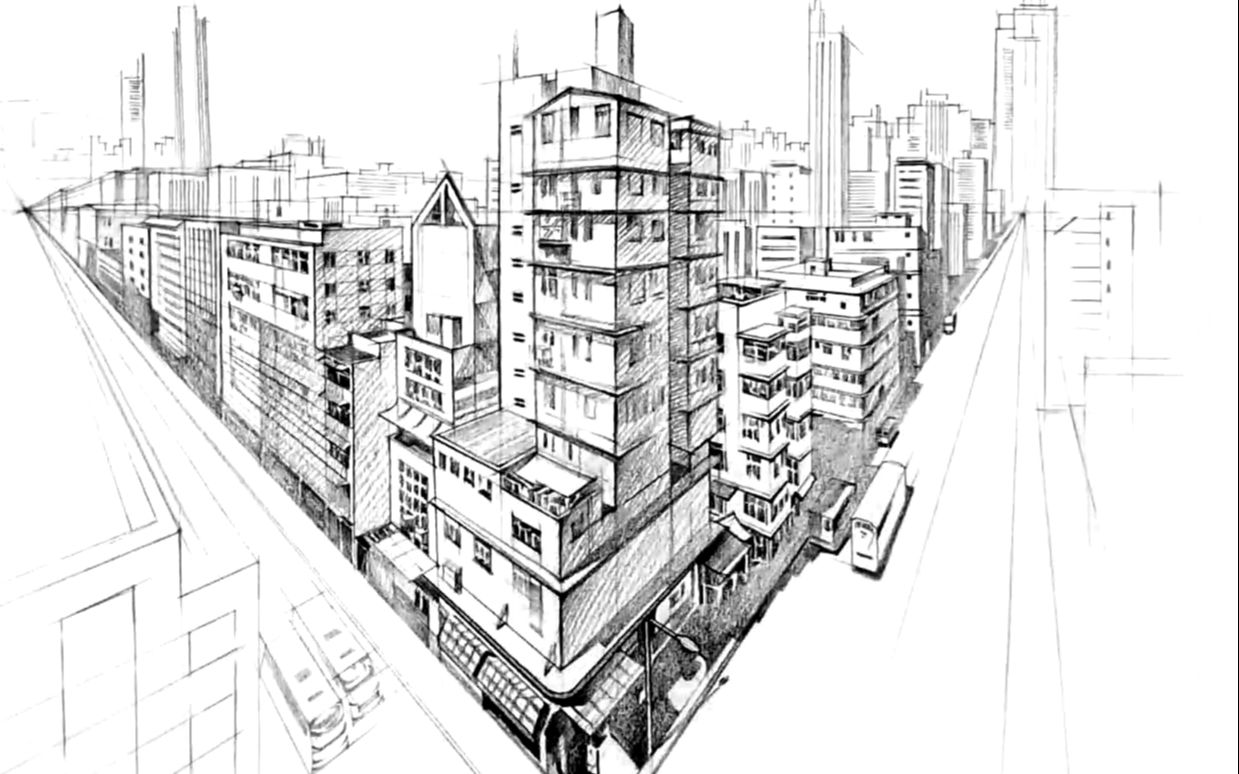
\includegraphics[width=0.4\linewidth]{pic/城市}
    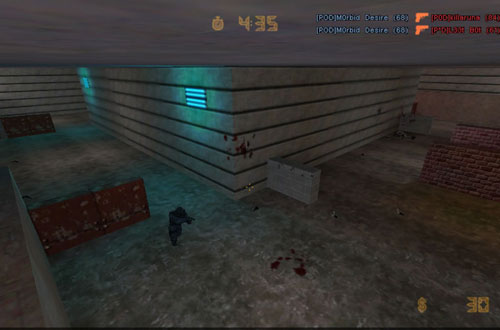
\includegraphics[width=0.4\linewidth]{pic/CS}
    \end{figure}

    二维图形变换矩阵表示
    \begin{equation*}
    \begin{pmatrix}x'\\y'\\\end{pmatrix}=
    \begin{pmatrix}a_{11}&a_{12}\\a_{21}&a_{22}\\\end{pmatrix}
    \begin{pmatrix}x\\y\\\end{pmatrix}+\begin{pmatrix}b_1\\b_2\\\end{pmatrix}
    \end{equation*}
    或者将上式齐次化表示为
    \begin{equation*}
    \begin{pmatrix}x'\\y'\\1\\\end{pmatrix}=
    \begin{pmatrix}
    a_{11}&a_{12}&b_{1}\\
    a_{21}&a_{22}&b_{2}\\
    0&0&1\\
    \end{pmatrix}
    \begin{pmatrix}x\\y\\1\\\end{pmatrix}
    \end{equation*}

    \blue{思考:} 旋转和平移变换分别对应那个矩阵?

    \end{frame}






\begin{frame}\frametitle{计算机绘图与图像变换*}
    相应的三维图像变换一般可表示为
    \begin{equation*}
    \begin{pmatrix}x'\\y'\\z'\\1\\\end{pmatrix}=
    \begin{pmatrix}
    a_{11}&a_{12}&a_{13}&b_{1}\\
    a_{21}&a_{22}&a_{23}&b_{2}\\
    a_{31}&a_{32}&a_{33}&b_{3}\\
    0&0&0&1\\
    \end{pmatrix}
    \begin{pmatrix}x\\y\\z\\1\\\end{pmatrix}
    \end{equation*}
    对于立体图形,为了保持立体视觉效果,需要将其恰当的投影到平面上.
    \begin{itemize}
    \item 中心投影: 例如以点$A(a,b,c)$为中心,坐标平面Oxy为投影平面. 则中心投影变换公式为
    \begin{equation*}
    \begin{pmatrix}x'\\y'\\z'\\w'\\\end{pmatrix}=
    \begin{pmatrix}
    c&0&a&0\\0&c&-b&0\\0&0&0&0\\0&0&-1&c\\
    \end{pmatrix}
    \begin{pmatrix}x\\y\\z\\w\\\end{pmatrix}
    \end{equation*}
    \item 平行投影: 沿着向量$(\alpha,\beta,\gamma)$投影到$Oxy$平面
    \begin{equation*}
    \begin{pmatrix}x'\\y'\\z'\\w'\\\end{pmatrix}=
    \begin{pmatrix}
    1&0&-\frac\alpha\gamma&0\\0&1&-\beta/\gamma&0\\0&0&0&0\\0&0&0&1\\
    \end{pmatrix}
    \begin{pmatrix}x\\y\\z\\w\\\end{pmatrix}
    \end{equation*}
    \end{itemize}

    注:这里都是用齐次坐标表示.

    \end{frame}





    \subsection{最小二乘法与奇异值分解*}
\begin{frame}\frametitle{最小二乘法与奇异值分解*}
    \begin{question}
    给定一组观测数据
    \[(x_i,y_i),\quad i=1,2,\cdots,n.\]
    寻找一个合适的函数$y=f(x)$使得函数图像尽量与观测数据贴合.
    \end{question}

    核心问题是如何用数学语言表述图像与观测数据贴合. 一种方便的策略是取 $f(x)$为不超过给定次数的多项式
    \[f(x)= a_0+a_1x+\cdots+a_{m-1}x^{m-1}\]
    使得
    \[g(a_0,a_1,\cdots,a_{m-1}):=\sum_{i=1}^n (f(x_i)-y_i)^2\]
    尽量小.基于该准则求拟合多项式$f(x)$的方法称为最小二乘法.
    \end{frame}





\begin{frame}\frametitle{最小二乘法与奇异值分解*}
    由 $\frac{\partial g}{\partial a_k}=0$, $k=0,1,\cdots,m-1$ 的到关于$a_0,a_1,\cdots,a_{m-1}$的线性方程组:
    \[AA^Ta=Ay \qquad (*)\]
    其中
    \begin{equation*}
    A=\begin{pmatrix}
    1&1&\cdots&1\\x_1&x_2&\cdots&x_n\\\vdots&\vdots&&\vdots\\x_1^{m-1}&x_2^{m-1}&\cdots&x_n^{m-1}\\
    \end{pmatrix},
    \quad
    a=\begin{pmatrix}a_0\\a_1\\\vdots\\a_{m-1}\\\end{pmatrix},
    \quad
    y=\begin{pmatrix}y_1\\y_2\\\vdots\\y_{n}\\\end{pmatrix}
    \end{equation*}

    分情况讨论:

    \begin{itemize}
    \item $n\geq m$: $AA^T>0$. 式$(*)$有唯一解.
    \item $n<m$: 对$A$进行奇异值分解. 即$A=PDQ$, 其中$P$, $Q$为正交矩阵, $D=\mathrm{diag}(\sigma_1,\cdots,\sigma_r,O_{(m-r)\times(n-r)})$(正交相抵标准形).
    \end{itemize}
    线性方程组(*)化简为
    \[DD^Tx=Dc\]
    其中$x=P^Ta$, $c=Qy$.于是$x_i = \frac{c_i}{\sigma_i}$, $i=1,2,\cdots,r$.于是
    \[a = P\left(\frac{c_1}{\sigma_1},\cdots,\frac{c_r}{\sigma_r},*\cdots,*\right)^T.\]
    特别地, $a=P\left(\frac{c_1}{\sigma_1},\cdots,\frac{c_r}{\sigma_r},0,\cdots,0\right)^T$为模长最小的解.
    \end{frame}





    \subsection{数字图像的压缩*}
\begin{frame}\frametitle{数字图像的压缩*}
    在不明显降低图像的视觉质量的基础上,jpeg格式对静止图片的压缩比一般可达$10:1\sim 50:1$.
    \begin{itemize}
    \item 分割成$8\times8$的子块 $A=(A_{ij})_{p\times q}$
    \item 离散余弦变换的 $B=PAP^T$其中$P=(p_{ij})_{8\times 8}$正交,$p_{1j}=\frac{1}{\sqrt{8}}$, $p_{ij}=\frac12\cos\frac{(i-1)(2j-1)\pi}{16}$ ($i\geq2$).
    \item 对$B_{ij}$(按某种方式)取整;
    \item 然后编码为长度不等的二进制数$c_{ij}$
    \item 最后得到编码系数矩阵$C=(c_{ij})_{p\times q}$.

    \end{itemize}
    \bigskip
    JPEG效果好在于$B_{ij}$是稀疏的. 即除了左上角少数元素除外,大多数元素绝对值都相当小.

    \bigskip
    图像压缩的基本方法: 寻找图像空间的一组基使得图像在这组基下的坐标为稀疏矩向量.
    \end{frame}





    \subsection{投入产出模型*}
\begin{frame}\frametitle{投入产出模型*}
    经济学家 Leontief 提出投入产出模型: 设经济社会中共有$n$中产品$P_1,P_2,\cdots,P_n$每生产一个单位的$P_i$需消耗$a_ij$个单位的$P_j$,矩阵$A=(a_{ij})_{n\times n}$称为消耗系数矩阵\footnote{为保可持续发展,须满足 $x \geq xA$,其中$x$为产出总量($y=xA$为投入总量).}.

    \begin{question}
    若以$f(x)=\min_{1\leq i\leq n}\frac{x_i}{y_i}$作为衡量生成效率的标准, $x$取何值时$f(x)$最大?
    \end{question}
    \yang{证明思路: 由Perron-Frobenius定理\footnote{不可拆分非负实方阵的最大模长特征值为正,重数为$1$且对应正特征向量. 不可拆分意思是不存在产品的重排使得$A$为准三角矩阵.},得$\lambda_1 x\geq xA$ 且等号成立当且仅当 $x$取对应特征向量.}
    \end{frame}





    \subsection{Markov矩阵*}
\begin{frame}\frametitle{Markov矩阵*}
    \begin{question}
    一个点在某网络中随机游走,在给定点出现的概率问题.
    \end{question}

    记从$i$点(随机)游走一步,到达$j$点的概率记为$m_{ij}$.则 $M=(m_{ij})_{n\times n}$为 Markov矩阵\footnote{满足$A(1,\cdots,1)^T=(1,1,\cdots,1)^T$的非负矩阵$A$,称为Markov矩阵.}.

    \begin{theorem} Markov矩阵$M=(m_{ij})_{n\times n}$有如下性质:
    \begin{enumerate}
    \item 若行向量$x$是$n$维概率向量,则$xM$也是$n$维概率向量.
    \item $1$是$M$的最大特征值, $n$为全$1$向量是对应的特征向量.
    \item 若对任意正整数$k$,$M^k$不可拆分,则$\lim_{k\to\infty}M^k=\textbf{1}\cdot c^T$,其中$c$为$M^T$属于$1$的特征向量.
    \end{enumerate}
    \end{theorem}
    \end{frame}





    \subsection{Google 搜索排序*}
\begin{frame}\frametitle{Google 搜索排序*}
    PageRank算法\footnote{Brin-Page 发明,并依此创立google.}根据网站内外链接的数量和质量来算网页的Pagerank.
    \begin{definition}
    \blue{假设}有$n$个网页,某网民在任意时刻都仅打开一个页面.假设他点击链接的概率是$\omega$,而关闭当前页面的概率为$1-\omega$. 在无限长时间后的某个时刻网页$P_j$被访问的概率为$p_j$就被称为是他的Pagerank.
    \end{definition}

    首先,构造邻接矩阵\footnote{$0$表示无连接,$1$表示有连接.}$A=(a_{ij})_{n\times n}$.
    Bayes 全概率公式
    \[p_j = \frac{1-\omega}{n} + \omega\sum_{i=1}^n p_i\frac{a_{ij}}{d_i}.\]
    解得 (其中 $D=\mathrm{diag}(d_1,\cdots,d_n)$, $p=(p_1,\cdots,p_n)$, $\textbf{1}=(1,\cdots,1)$)
    \[p=\frac{1-\omega}{n}\textbf{1}\left(1-\omega D^{-1}A\right)^{-1}.\]
    注: 实际问题中$n$很大,用Gauss消元法或计算逆矩阵的方法求解计算量为$O(n^3)$,几乎不可能实现.

    由于$D^{-1}A$为Markov矩阵,其特征值模都不超过$1$. 在Pagerank算法中,取 $\omega=0.85$,因此
    \[\left(1-\omega D^{-1}A\right)^{-1} = \sum_{i=0}^\infty \left(\omega D^{-1}A\right)^i.\]
    \end{frame}





\subsection{层次分析法*}
\begin{frame}\frametitle{层次分析法*}
    层次分析是决策论中一种重要的方法.

    设系统共有$m$层因素,第$k$层有$n_k$个. 第$k$层的第$i$个因素受第$k+1$层的第$j$个因素的影响程度为$p_{k,i,j}$.则目标层受方案层的影响程度可通过矩阵
    \[P = P_1P_2\cdots P_{m-1}\]
    来表示.

    注:矩阵$P_k$比较难确定.但比较矩阵\footnote{$b^{ki}_{j_1j_2}=\frac{p_{k,i,j_1}}{p_{k,i,j_2}}$} $B^{k\ell}=(b^{ki}_{j_1j_2})$比较好估计.

    \begin{enumerate}
    \item 估算$B$
    \item 求方程组$\left\{\frac{x_i}{x_j}=b_{ij},i,j=1,2,\cdots,n_{k+1}\right\}$的最小二乘解\footnote{需要用到行主对角占优矩阵的性质}.
    \item 令$P_k$的第$\ell$行为$x$.计算$P$.
    \end{enumerate}
    \begin{theorem}
    若$A$可逆,主对角占优($a_{ii}\geq\sum_{j\neq i}|a_{ij}|$)且$a_{ij}<0$($\forall i\neq j$),则$A^{-1}$的每个元素都为正数.
    \end{theorem}
    \end{frame}









